\documentclass[10pt]{article}
\usepackage[utf8]{inputenc}
\usepackage{amscd}
\usepackage{amsmath}
\usepackage{amssymb}
\usepackage{amsthm}
\usepackage{listings}
\usepackage{enumerate}
\usepackage{graphicx}

\textwidth=15cm \textheight=22cm \topmargin=0.5cm \oddsidemargin=0.5cm \evensidemargin=0.5cm

\graphicspath{{images/}}

\newcommand{\sk}{\vskip 10mm}
\newcommand{\bb}[1]{\mathbb{#1}}
\newcommand{\ra}{\rightarrow}

\theoremstyle{plain}
\newtheorem{problem}{Problem}
\newtheorem{lemma}{Lemma}[problem]

\theoremstyle{remark}
\newtheorem{tpart}{}[problem]
\newtheorem*{ppart}{}

\begin{document}

\begin{problem}
  On the 2-sphere, consider the flow
  \[
    \theta(t,\langle x,y,z\rangle)
    =\langle x,y\cos(t)-z\sin(t),y\sin(t)+z\cos(t)\rangle
  \]
  Find the vector field on $S^2$ induced by this flow.
\end{problem}

Take the derivative of $\theta$ with respect to time to get
\[
  \frac{\partial \theta}{\partial t}(\langle x,y,z\rangle) = \langle 0,-y\sin(t)-z\cos(t),y\cos(t)-z\sin(t)\rangle
\]
Then set $t=0$ to get the vector field
\[
  \xi(\langle x,y,z\rangle) = \langle 0,-z,y\rangle
\]
on $S^2$ corresponding to the flow $\theta$.

\sk

\begin{problem}
  Consider the vector field $\xi(x)=x$ on $\bb{R}$. Show that $\xi$ is the
  tangent field to a flow, and find the flow. (Hint: In classical notation,
  this vector field corresponds to the initial value problem $dy/dt=y,y(0)=x$.)
\end{problem}

If we solve the differential equation $\frac{dy}{dt}=y$ we get
$y=Ae^t$. Solving for initial conditions we get
\[
  \theta(t,x)=xe^t
\]
as our flow.

\sk

\begin{problem}[4]
  If $X$ and $Y$ vector fields on $M$ then $XY$ makes sense as an operator
  on smooth real valued functions on $M$. Show that $[X,Y]=XY-YX$ is a vector
  field. (This is called the ``Lie bracket'' of $X$ and $Y$. Sometimes it is
  defined with opposite sign.) Also show that $XY$ itself is not a vector
  field.
\end{problem}

\begin{proof}
  Let $X=a^i\frac{\partial}{\partial x_i}$ and $Y=b^i\frac{\partial}{\partial x_i}$ be vector fields and let
  $f$ be a smooth function. Then
  \[
    XYf = a^j\frac{\partial Yf}{x_j}=a^j\frac{\partial(b^i\frac{\partial f}{\partial x_i})}{\partial x_j}=a^j\left(\frac{\partial b^i}{\partial x_j}\frac{\partial f}{\partial x_i}+b^i\frac{\partial^2 f}{\partial x_i\partial x_j}\right) = a^j\frac{\partial b^i}{\partial x_j}\frac{\partial f}{\partial x_i}+a^ib^i\frac{\partial^2 f}{\partial x_i\partial x_j}
  \]
  and similarly
  \[
    YXf = b^j\frac{\partial a^i}{\partial x_j}\frac{\partial f}{\partial x_i}+b^ia^i\frac{\partial^2 f}{\partial x_i\partial x_j}
  \]
  Then the Lie bracket of $X$ and $Y$ is
  \[
    [X,Y]f=XYf-YXf=a^j\frac{\partial b^i}{\partial x_j}\frac{\partial f}{\partial x_i}+a^ib^i\frac{\partial^2 f}{\partial x_i\partial x_j}-b^j\frac{\partial a^i}{\partial x_j}\frac{\partial f}{\partial x_i}+b^ia^i\frac{\partial^2 f}{\partial x_i\partial x_j} = \left(a^j\frac{\partial b^i}{\partial x_j}-b^j\frac{\partial a^i}{\partial x_j}\right)\frac{\partial f}{\partial x_i}
  \]
  which shows that $[X,Y]$ is in fact a vector field.
\end{proof}

From the above calculation one can see that $XY$ is not a vector field as
\[
  XYf = a^j\frac{\partial b^i}{\partial x_j}\frac{\partial f}{\partial x_i}+a^ib^i\frac{\partial^2 f}{\partial x_i\partial x_j}
\]
which is not in the proper form to be a vector field.

\pagebreak

\begin{problem}[5]
  Show that the Klein Bottle has an everywhere nonzero vector field.
  Describe the resulting flow.
\end{problem}

\begin{center}
  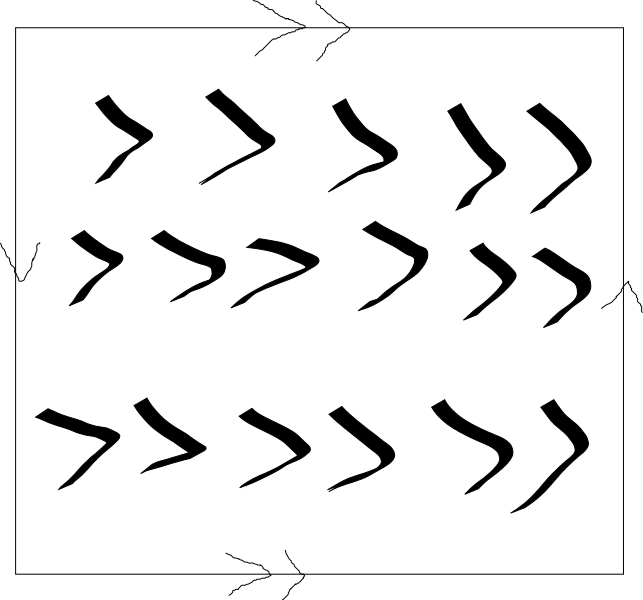
\includegraphics[scale=.5]{klein}  
\end{center}
%%%%%%%%%%%%%%%%%%%%%%%%%%%%%%%%%%%%%%%%%%%%%%%%%%%%%%%%%%%%%%%%%%%%%%%%%%%%%
\end{document}
